\section{Architektur}

\begin{figure}[h]
    \centering
    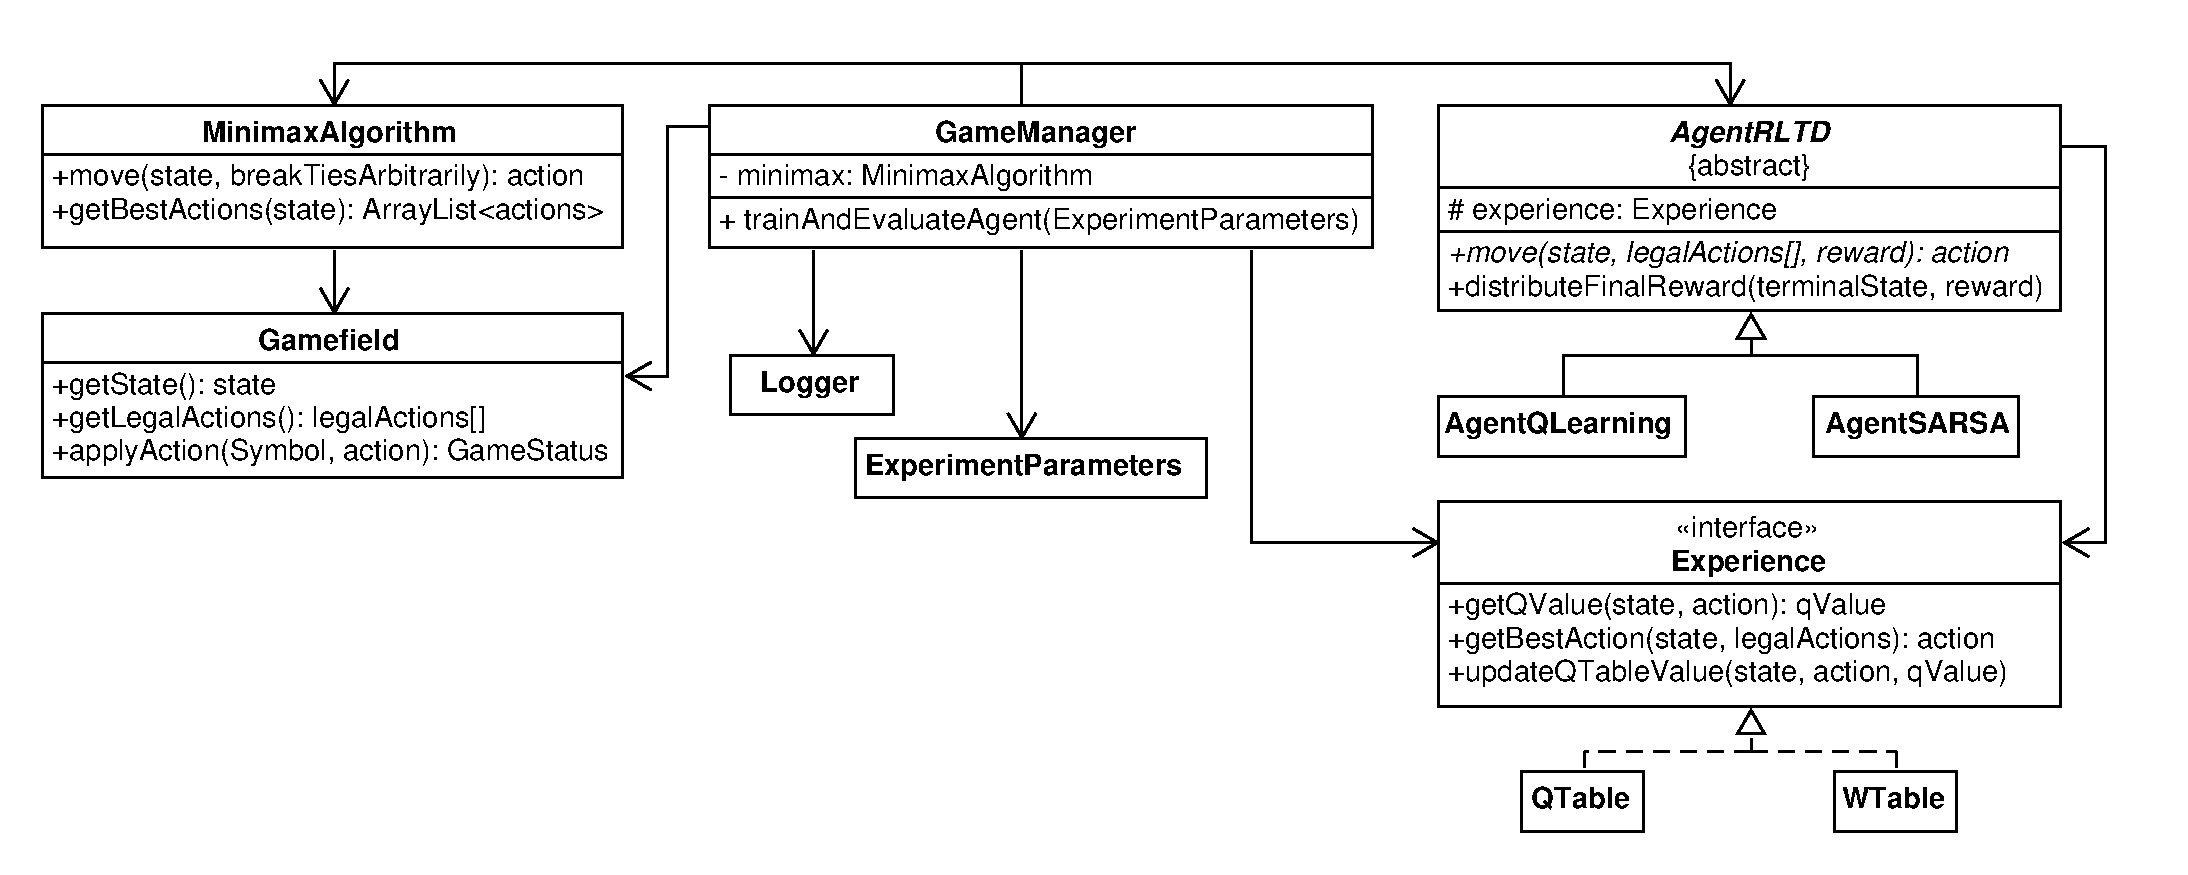
\includegraphics[width=\linewidth]{uml/uml_architektur.pdf}
    \caption{Grobe Übersicht der wichtigsten Klassen und deren Interaktion}
    \label{fig:uml_architektur}
\end{figure}

In \cref{fig:uml_architektur} ist eine Übersicht der wichtigsten Klassen.
Das UML-Diagramm stellt keinen Anspruch an Vollständigkeit, sondern dient der Vermittlung eines grundlegenden Verständnisses für die wichtigsten Bestandteile der Anwendung sowie deren Interaktion. 
Der GameManager ist die zentrale Klasse, die alle anderen Klassen verbindet, um Training und Evaluation der Agenten durchzuführen.  
Auf Basis, der in ExperimentParameters definierten Werte erstellt der GameManager zwei Agenten und weist diesen eine gemeinsame Experience Instanz zu. 
Die beiden Agenten werden mittels \splay trainiert und anschließend in Evaluationsspielen getestet. 
Zur Bewertung der Agenten verwendet der GameManager den Minimax-Algorithmus. 
Währenddessen erstellt der GameManager Log-Dateien auf deren Basis die Auswertung erfolgt.
Einerseits CSV-Dateien, die zum Plotten der Konvergenz und Berechnen der Spielstärke verwendet werden.
Zum anderen Dateien, wie im \cref{chap:meta}, die für Training und Evaluation verwendete Experimentparameter und Spielergebnisse enthalten. 
In den folgenden Abschnitten werden die Bestandteile genauer betrachtet.

Für die Implementierung wurde Java 16 und somit die derzeit aktuellste Java Version verwendet. 
Um die volle Kontrolle über die Implementierung der Agenten zu haben, wurden keine zusätzlichen Bibliotheken eingebunden. 
Die einzige Ausnahme ist die Bibliothek Apache CommonsCSV, die zur Erstellung von CSV-Dateien genutzt wird. 
Der Source-Code und die Dokumentation der Anwendung sowie Verwendungshinweise werden bereitgestellt auf \href{http://github.com/JonasBingel/ThesisHSMZ-RLTicTacToe-Java}{Github.com/JonasBingel}